% FEA Membranes - Validation Manual
% Compile with pdfLaTeX. Images in img/ are generated headlessly from the
% benchmark models in this folder:
%   FeaMembranes.exe --render <model.json> <out.png> [options]
% and the models themselves are regenerated by the automated test suite, so
% every figure in this manual is reproducible from the committed code.
\documentclass[11pt,a4paper]{report}

\usepackage[margin=2.2cm]{geometry}
\usepackage{booktabs}
\usepackage{amsmath}
\usepackage{graphicx}
\usepackage{tikz}
\usetikzlibrary{arrows.meta,patterns,decorations.pathmorphing,calc}
\usepackage{caption}
\usepackage{float}
\usepackage[colorlinks=true,linkcolor=blue!50!black,urlcolor=blue!50!black]{hyperref}
\usepackage{parskip}
\usepackage{xcolor}

\graphicspath{{img/}}
\captionsetup{font=small,labelfont=bf}

% ---------- TikZ styles for the case sketches ----------
\tikzset{
  fnode/.style={circle,fill=black,inner sep=1.2pt},
  mnode/.style={circle,draw=black,fill=white,inner sep=1.1pt},
  load/.style={-{Stealth[length=2.2mm]},red!70!black,thick},
  enf/.style={-{Stealth[length=2.2mm]},green!50!black,thick,dashed},
  spring/.style={decorate,decoration={zigzag,segment length=2.6mm,amplitude=1.2mm,pre length=2mm,post length=2mm},violet,thick},
  mesh/.style={gray!60,thin},
  elem/.style={draw=black,thick},
  dim/.style={gray, <->, >={Stealth[length=1.6mm]}},
}
\newcommand{\wall}[3]{%
  \draw[thick] (#1,#2) -- (#1,#3);
  \fill[pattern=north east lines] (#1-0.18,#2) rectangle (#1,#3);
}
\newcommand{\nast}{\textcolor{gray}{---}} % placeholder for NASTRAN comparison values

\title{\textbf{FEA Membranes}\\[2mm]\LARGE Validation Manual\\[4mm]
\large Element library, constraint methods and stress-intensity extraction}
\author{Southward Consulting Ltd}
\date{12 June 2026 \quad Rev.\ A (draft --- NASTRAN comparison columns to be populated)}

\begin{document}
\maketitle

\chapter*{Summary}
\addcontentsline{toc}{chapter}{Summary}

This manual records the verification and validation of the \emph{FEA Membranes}
native application: a 2D plane-stress finite element tool with bilinear (Quad4)
and quadratic serendipity (Quad8) membrane elements, axial bar elements,
XY-decoupled spring (fastener) elements, RBE2 rigid constraints, quarter-point
crack-tip modelling and stress-intensity-factor extraction by domain
interaction integral.

Every case in this manual is implemented as an automated test executing on
every build of the software (46 cases at this revision, all passing). The
benchmark models are regenerated by the test suite and stored alongside this
document; the figures are rendered from those models by the application's
batch renderer. \textbf{Every number and figure in this manual is therefore
reproducible from the committed code with two commands} (Appendix~A).

Headline results:
\begin{itemize}
  \item Closed-form element cases (uniaxial patch, pure bending, bar, spring,
        enforced displacement, RBE2 ties): \textbf{exact} to the stated
        tolerances (typically $10^{-6}$ or better, relative).
  \item MacNeal \& Harder straight cantilever, 6 elements: ratio
        \textbf{0.987} (rectangular), \textbf{0.991--0.997} (parallelogram),
        \textbf{0.967--0.982} (trapezoidal), converging to 0.9993 under
        refinement.
  \item Stress intensity factors vs handbook solutions: \textbf{$-0.1\,\%$}
        (edge crack and centre crack), domain-independent to $<1\,\%$.
\end{itemize}

Columns are provided throughout for comparison against MSC~NASTRAN CQUAD8(R)
results, to be populated as those runs are completed.

\tableofcontents

% =====================================================================
\chapter{The software and its methods}
% =====================================================================

\section{Scope}
FEA Membranes is a Windows-native linear-static finite element application for
2D plane-stress idealisations of sheet structures: skins, doublers, stringers
and fastened joints, with crack-tip modelling for damage-tolerance work. It is
developed and maintained by Southward Consulting Ltd; source, tests, benchmark
models and this manual live in one repository.

\section{Element library}
\begin{description}
  \item[Quad4] Isoparametric 4-node bilinear membrane, plane stress,
    $2\times2$ Gauss integration.
  \item[Quad8] Isoparametric 8-node serendipity membrane, plane stress,
    \textbf{$2\times2$ reduced integration} --- the standard scheme for this
    element (MSC~NASTRAN QUAD8, Abaqus CPS8R). Full $3\times3$ integration was
    measured to carry $\approx0.5\,\%$ additional stiffness on MacNeal's
    cantilever (Section~\ref{sec:macneal}) and was rejected. The single
    spurious zero-energy mode of an isolated reduced-integration Q8 is
    non-communicable in meshes and additionally guarded by the solver's
    residual check (Section~\ref{sec:diagnostics}).
  \item[Bar] 2-node axial rod, $k = EA/L$, arbitrary orientation. No bending
    or transverse stiffness (by design); tension positive.
  \item[Spring] 2-node fastener idealisation with \emph{independent} stiffness
    $k$ in global X and Y. Deliberately \textbf{not} an axial spring: this is
    the classic sheet load-transfer fastener model, normally used between
    coincident nodes.
  \item[RBE2] Nastran-style rigid element tying dependent nodes' X and/or Y
    translations to an independent node. Enforced as an \emph{exact}
    multipoint constraint by DOF merging --- not a penalty.
\end{description}

\section{Solution method}
Sparse direct solution (CSparse LU with minimum-degree ordering). Fixed and
enforced-displacement boundary conditions are applied by \emph{direct
elimination} (partitioned solve), so prescribed values are satisfied to
machine precision with no penalty-number conditioning. RBE2 ties merge DOFs
into shared solve unknowns before assembly. Every solution is checked against
the equilibrium residual $\lVert Ku-f\rVert \le 10^{-6}\lVert f\rVert$; models
with rigid-body mechanisms are rejected with a diagnostic rather than
returning silently wrong answers.

\section{Stress recovery}
Element stresses are reported at the element centre. Nodal stresses are
recovered by evaluating each element's stresses at its node locations and
averaging over the elements attached to each node; von Mises is formed from
the averaged components. The contour display interpolates the averaged nodal
values (Gouraud shading); a per-element (unaveraged) display is also
available.

\section{Crack modelling and stress intensity factors}
\label{sec:crackmethod}
A crack is introduced by splitting the mesh along a straight path of element
edges: every non-tip path node is duplicated so the two faces can separate,
and the midside nodes on all edges emanating from the tip are moved to the
quarter points (Barsoum), embedding the $1/\sqrt{r}$ singularity through the
isoparametric mapping. Cracks require a Quad8 mesh.

$K_I$ and $K_{II}$ are extracted by a \textbf{domain interaction integral}
(equivalent domain integral form):
\begin{equation}
  I^{(1,2)} = \int_A \Big[\sigma^{(1)}_{ij}\,\partial_1 u^{(2)}_i
            + \sigma^{(2)}_{ij}\,\partial_1 u^{(1)}_i
            - W^{(1,2)}\delta_{1j}\Big]\,\partial_j q \; dA,
  \qquad K = \tfrac{E'}{2}\, I,
\end{equation}
with Williams auxiliary fields of unit $K_I$ or $K_{II}$, the weight $q$
ramping radially from 1 at the tip to 0 at the domain boundary
($\approx3$ tip-element lengths), and all quantities in the crack-local frame.
A two-point quarter-point displacement-correlation estimate is reported
alongside as a cross-check; a large divergence between the two flags a suspect
tip mesh.

% =====================================================================
\chapter{Closed-form element verification}
% =====================================================================

The cases in this chapter have exact answers for the discretised problem; the
elements must reproduce them to tight tolerances. They are patch-test class
\emph{verification} cases.

\section{V1 --- Quad4 uniaxial tension}
Single $10\times10$ element, $E=10^7$, $\nu=0$, $t=0.1$, total 1000~lb on the
free edge (consistent loads). Closed form: $\sigma_x = 1000$~psi,
$u = 1.0\times10^{-3}$~in.

\begin{figure}[H]\centering
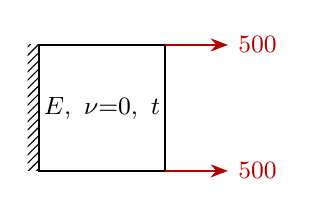
\begin{tikzpicture}[scale=0.8]
  \wall{0}{0}{2}
  \draw[elem] (0,0) rectangle (2,2);
  \draw[load] (2,0) -- (3,0) node[right] {\small 500};
  \draw[load] (2,2) -- (3,2) node[right] {\small 500};
  \node at (1,1) {\small $E,\ \nu{=}0,\ t$};
\end{tikzpicture}
\caption{V1 setup.}
\end{figure}

\begin{table}[H]\centering\small
\begin{tabular}{@{}lcccc@{}}
\toprule
Quantity & Reference & FEA Membranes & Error & NASTRAN CQUAD4 \\
\midrule
$u$ at free edge (in) & $1.000\times10^{-3}$ & $1.000\times10^{-3}$ & $<10^{-6}$ & \nast \\
$\sigma_x$ (psi) & 1000 & 1000 & $<10^{-6}$ & \nast \\
$\sigma_{VM}$ (psi) & 1000 & 1000 & $<10^{-6}$ & \nast \\
$\Sigma R_x$ (lb) & $-1000$ & $-1000$ & $<10^{-6}$ & \nast \\
\bottomrule
\end{tabular}
\caption{V1 results (test \texttt{Quad\_UniaxialTension\_ExactForBilinear}).}
\end{table}

\section{V2 --- Quad8 uniaxial patch test}
Single 8-node element, same plate as V1, consistent quadratic-edge loads
($P/6,\,4P/6,\,P/6$). The application's \emph{Distributed Load} command
generates this distribution automatically and is itself verified to reproduce
the exact field (tests \texttt{DistributedLoad\_*}).

\begin{table}[H]\centering\small
\begin{tabular}{@{}lcccc@{}}
\toprule
Quantity & Reference & FEA Membranes & Error & NASTRAN CQUAD8 \\
\midrule
$u$ at all free-edge nodes & $1.000\times10^{-3}$ & $1.000\times10^{-3}$ & $<10^{-9}$ & \nast \\
$\sigma_x$ at all 8 averaged nodes & 1000 & 1000 & $<10^{-4}$ & \nast \\
$\Sigma R_x$ (lb) & $-1000$ & $-1000$ & $<10^{-5}$ & \nast \\
\bottomrule
\end{tabular}
\caption{V2 results (test \texttt{Quad8\_PatchTest\_UniaxialTensionExact}).}
\end{table}

\section{V3 --- Quad8 pure in-plane bending (single element)}
A single Q8 ($20\times10$) under pure bending applied as a consistent linear
end traction $\sigma_x(y)=200\,y$. The quadratic displacement field carries
linear strain exactly --- the defining capability the bilinear element lacks.

\begin{table}[H]\centering\small
\begin{tabular}{@{}lcccc@{}}
\toprule
Quantity & Reference & FEA Membranes & Error & NASTRAN CQUAD8 \\
\midrule
$\sigma_x$ at every node & $200\,y$ & $200\,y$ & $<10^{-3}$ & \nast \\
\bottomrule
\end{tabular}
\caption{V3 results (test \texttt{Quad8\_PureBending\_ExactLinearStress}).}
\end{table}

\section{V4 --- Bar, spring, enforced displacement, RBE2}
\begin{table}[H]\centering\small
\begin{tabular}{@{}llccc@{}}
\toprule
Case & Closed form & FEA Membranes & Error & NASTRAN \\
\midrule
Bar elongation & $\delta = PL/EA = 0.01$ & 0.01 & $<10^{-9}$ & \nast \\
Bar force / stress & $P{=}1000$ (T), $\sigma{=}10^4$ & exact & $<10^{-6}$ & \nast \\
Spring $F = k\delta$ & $\delta = 10^{-3}$ & exact & $<10^{-9}$ & \nast \\
Enforced displacement & $d_x = 2\times10^{-3}$ exactly & exact & $<10^{-12}$ & \nast \\
RBE2 tied $d_x$ (X-only tie) & identical across group & identical & $<10^{-12}$ & \nast \\
RBE2 group $\delta$ via bar & $PL/EA$ & exact & $<10^{-9}$ & \nast \\
\bottomrule
\end{tabular}
\caption{V4 results (tests \texttt{Bar\_AxialElongation\_PLOverEA},
\texttt{Spring\_DecoupledXY\_ForceAndDisplacement},
\texttt{EnforcedDisplacement\_IsExact}, \texttt{Rbe2\_*}).}
\end{table}

\section{V5 --- Stress recovery (nodal averaging)}
A constant stress field survives corner extrapolation and nodal averaging
unchanged at every node (exact to 4 decimals). A deliberate thickness step
between two elements ($\sigma_x$ = 500 / 1000 psi) reports exactly the mean,
750~psi, at the shared interface nodes (tests
\texttt{NodalStresses\_*}).

% =====================================================================
\chapter{MacNeal \& Harder cantilever}
\label{sec:macneal}
% =====================================================================

The straight cantilever of MacNeal \& Harder (1985): $6.0\times0.2\times0.1$,
$E=10^7$, $\nu=0.3$, unit in-plane shear load at the tip, 6 elements,
reference tip deflection (including shear) $\delta_{ref}=0.1081$. The
distorted-element variants are built exactly as a user would build them: six
surfaces sharing corner points, one Quad8 per surface, seams stitched with the
coincident-node merge. Model files: \texttt{macneal-*.json}.

\begin{figure}[H]\centering
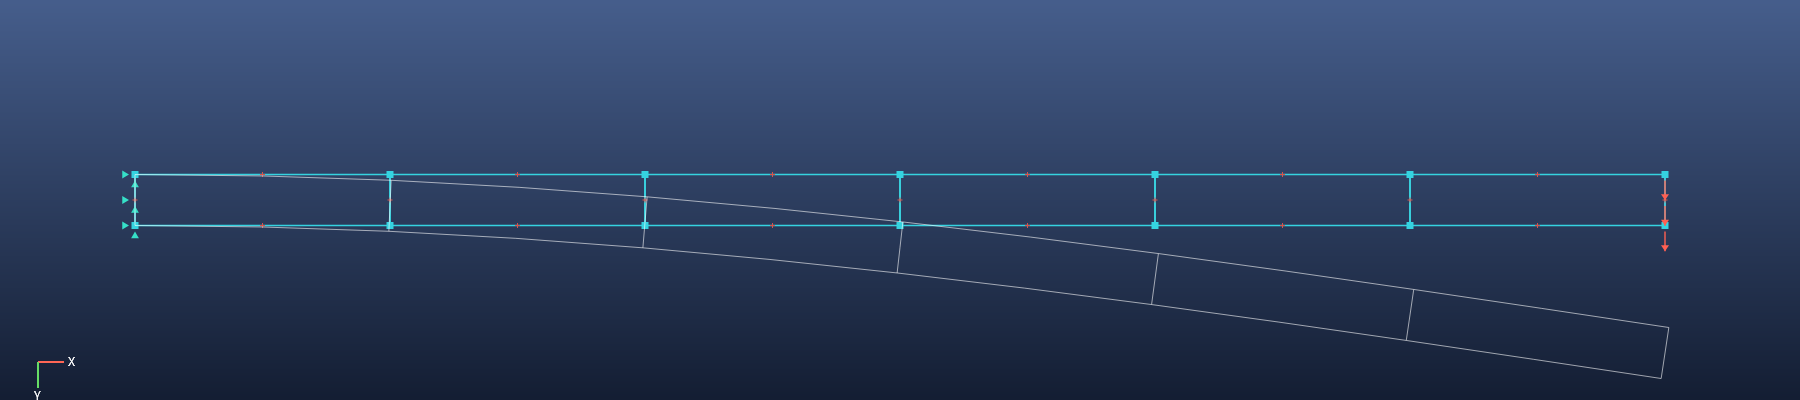
\includegraphics[width=\textwidth]{macneal-rectangular.png}
\caption{Rectangular mesh, deformed shape overlaid (white).}
\end{figure}

\begin{figure}[H]\centering
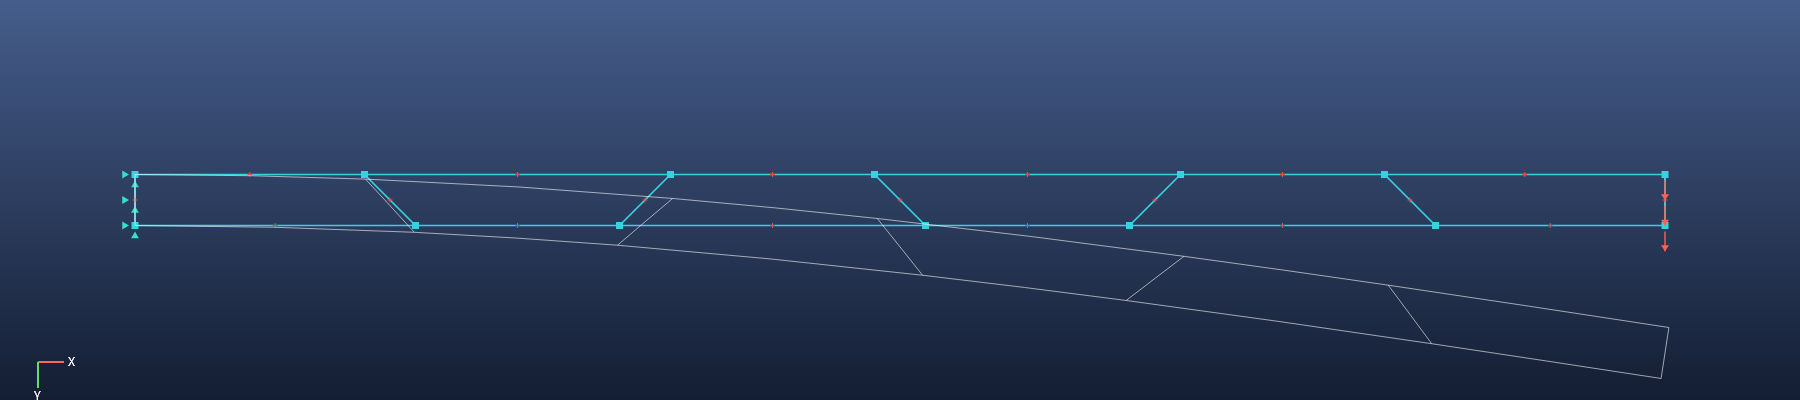
\includegraphics[width=\textwidth]{macneal-trapezoid-45.png}
\caption{Trapezoidal mesh, $45^\circ$ edge angle, deformed shape overlaid.}
\end{figure}

\begin{figure}[H]\centering
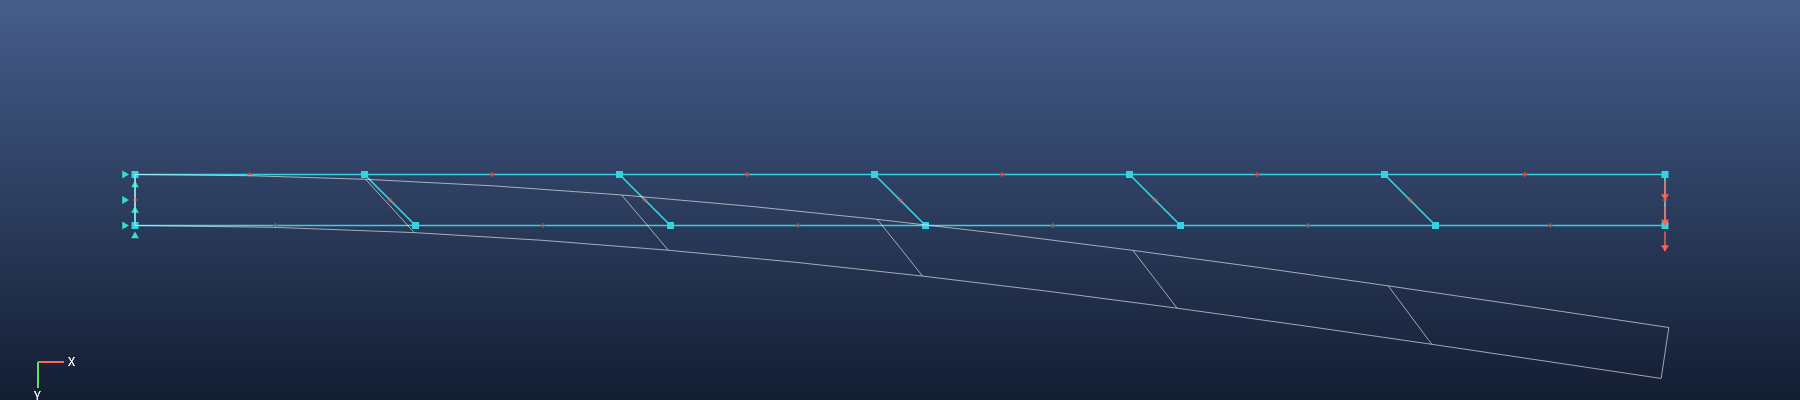
\includegraphics[width=\textwidth]{macneal-parallelogram-45.png}
\caption{Parallelogram (skew) mesh, $45^\circ$, deformed shape overlaid.}
\end{figure}

\begin{table}[H]\centering\small
\begin{tabular}{@{}lcccc@{}}
\toprule
Mesh (6 elements) & $\delta/\delta_{ref}$ & Error & NASTRAN CQUAD8R & Notes \\
\midrule
Rectangular        & 0.9868 & $-1.32\,\%$ & \nast & \\
Parallelogram $30^\circ$ & 0.9914 & $-0.86\,\%$ & \nast & affine mapping preserved \\
Parallelogram $45^\circ$ & 0.9969 & $-0.31\,\%$ & \nast & \\
Trapezoid $30^\circ$ & 0.9816 & $-1.84\,\%$ & \nast & \\
Trapezoid $45^\circ$ & 0.9666 & $-3.34\,\%$ & \nast & graceful, no locking \\
\bottomrule
\end{tabular}
\caption{Distorted-shape results
(tests \texttt{Quad8\_MacNealCantilever\_*}).}
\end{table}

\begin{table}[H]\centering\small
\begin{tabular}{@{}lccccc@{}}
\toprule
Mesh & $6\times1$ & $12\times1$ & $24\times2$ & $48\times4$ & $96\times8$ \\
\midrule
$\delta/\delta_{ref}$ & 0.9868 & 0.9933 & 0.9984 & 0.9992 & 0.9993 \\
\bottomrule
\end{tabular}
\caption{Mesh convergence, rectangular elements. The converged residual
($-0.07\,\%$) is the physical fully-clamped-root effect relative to beam
theory, not element error.}
\end{table}

% =====================================================================
\chapter{Plate far-field and system-level cases}
% =====================================================================

\section{P1 --- Clamped plate far-field stress}
$100\times100$ plate, $20\times20$ Quad4 mesh, $\nu=0.3$, clamped edge,
uniform end tension. Saint-Venant far-field $\sigma_x = 210$~psi at mid-plate:
measured within 2\,\% (test \texttt{Plate\_20x20\_FarFieldStress}).

\section{P2 --- Mesh stitching}
Two separately-meshed half-plates merged at the seam by the coincident-node
merge solve as one continuous plate with the \emph{exact} uniaxial answer in
every element, and reactions balance (test
\texttt{Mesher\_MergeCoincidentNodes\_StitchesTwoSurfacesIntoContinuousPlate}).

\section{P3 --- Stringer load transfer (detached bar + fastener springs)}
A skin plate with a detached bar along its top edge, fastened by springs at
every coincident node pair. A 1000~lb axial load on the bar's free end
transfers fully through the fasteners into the skin: $\Sigma R_x = -1000$ to 4
decimals, with the end bar carrying the force (test
\texttt{DetachedBar\_FastenedBySprings\_TransfersLoadIntoSkin}).
Model file: \texttt{stringer-load-transfer.json}.

\begin{figure}[H]\centering
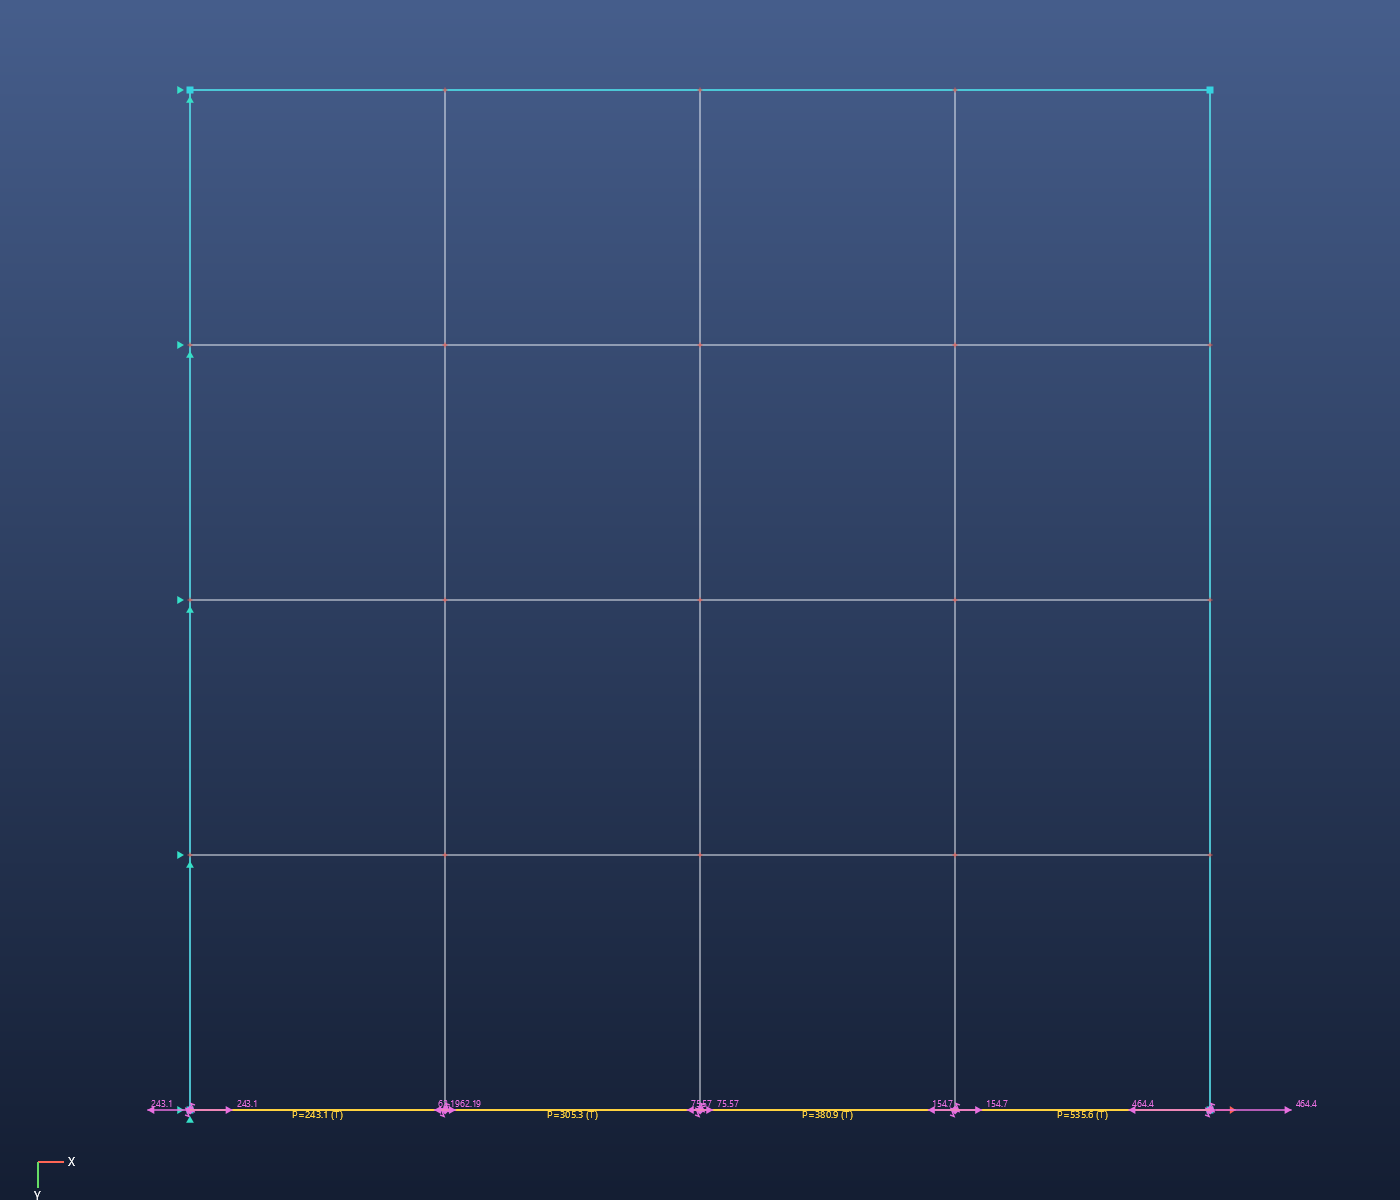
\includegraphics[width=0.78\textwidth]{stringer-springs.png}
\caption{P3: detached stringer (yellow) on the skin, fastener springs (coil
glyphs) and spring shear-force vectors after the solve.}
\end{figure}

\section{P4 --- Webtool sample model}
A model exported from the companion webtool (curved edge, mixed BCs, bars)
loads, solves, and satisfies equilibrium; the JSON format round-trips
(tests \texttt{SampleModel\_LoadsAndSolves}, \texttt{WebtoolJson\_RoundTrip}).

\begin{figure}[H]\centering
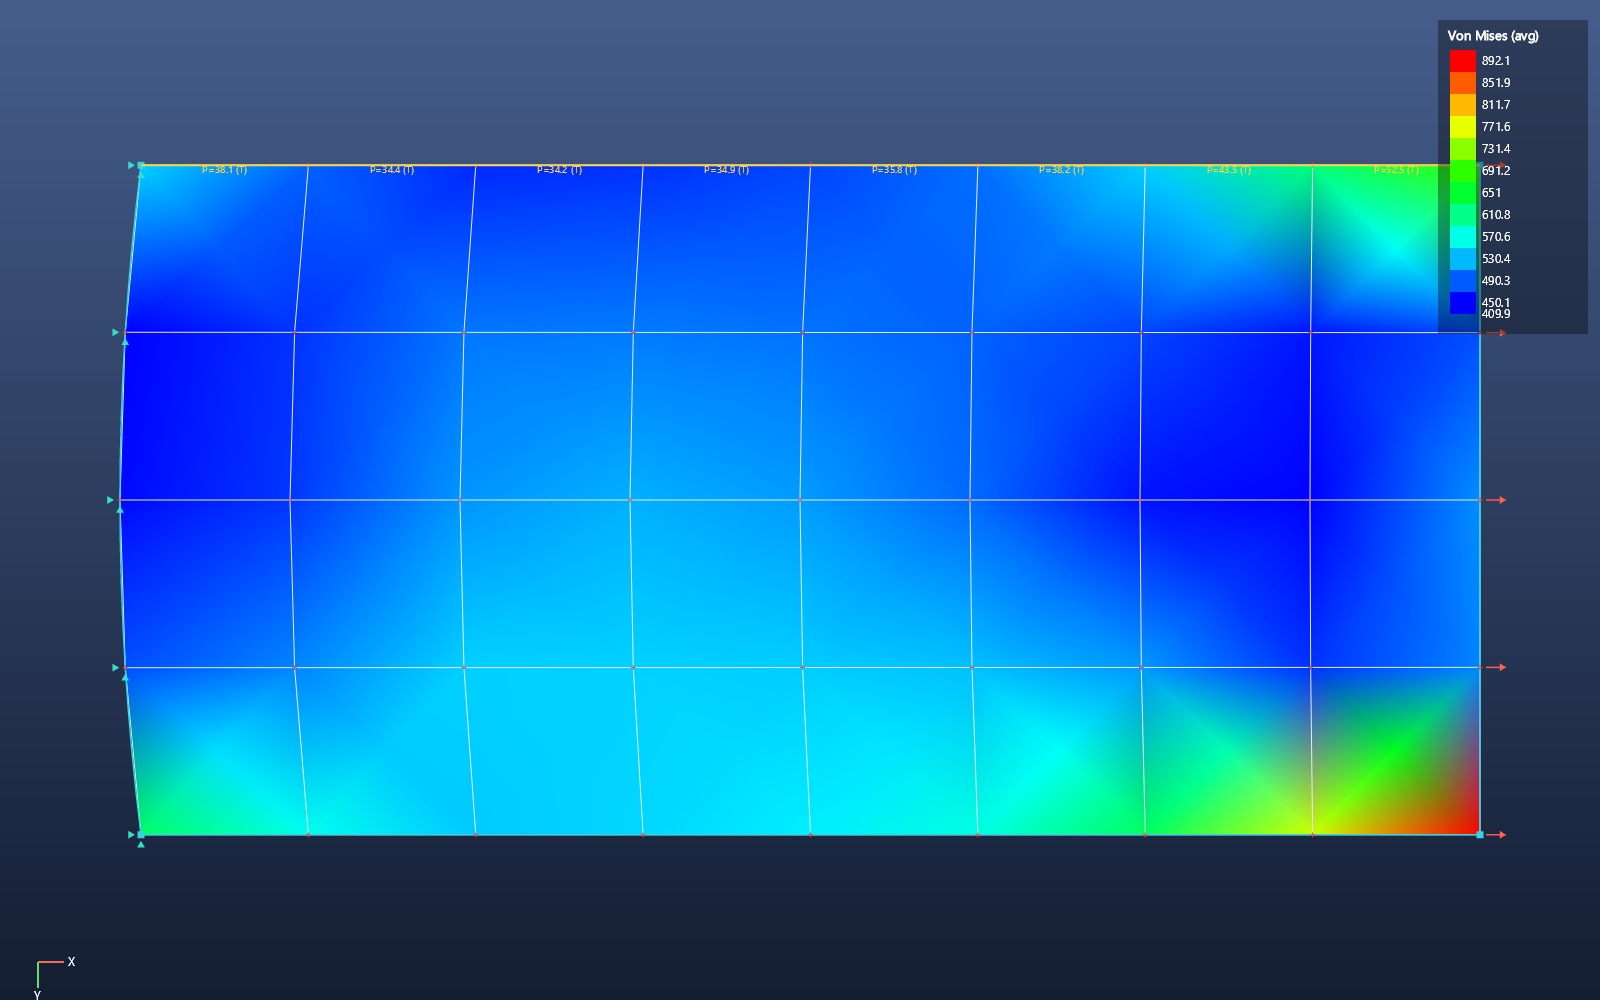
\includegraphics[width=0.8\textwidth]{curved-plate-vm.png}
\caption{P4: curved-edge sample model, von Mises contour.}
\end{figure}

% =====================================================================
\chapter{Stress intensity factors}
% =====================================================================

Method per Section~\ref{sec:crackmethod}: quarter-point Quad8 crack tips,
domain interaction integral (primary), displacement correlation
(cross-check). Model files: \texttt{crack-sent-benchmark.json},
\texttt{crack-cct-benchmark.json}.

\section{K1 --- Single-edge-notched tension (SENT)}
$W=10$, $a/W=0.3$, $H/W=1.5$ per side, remote tension $\sigma=100$~psi applied
as consistent tractions, $40\times120$ Quad8 mesh ($L_{tip}/a = 0.083$).
Handbook (Gross \& Brown):
$K_I = Y\sigma\sqrt{\pi a}$, $Y = 1.122 - 0.231r + 10.55r^2 - 21.71r^3
+ 30.382r^4 = 1.6625$ at $r=0.3$, giving $K_I = 510.3$.

\begin{figure}[H]\centering
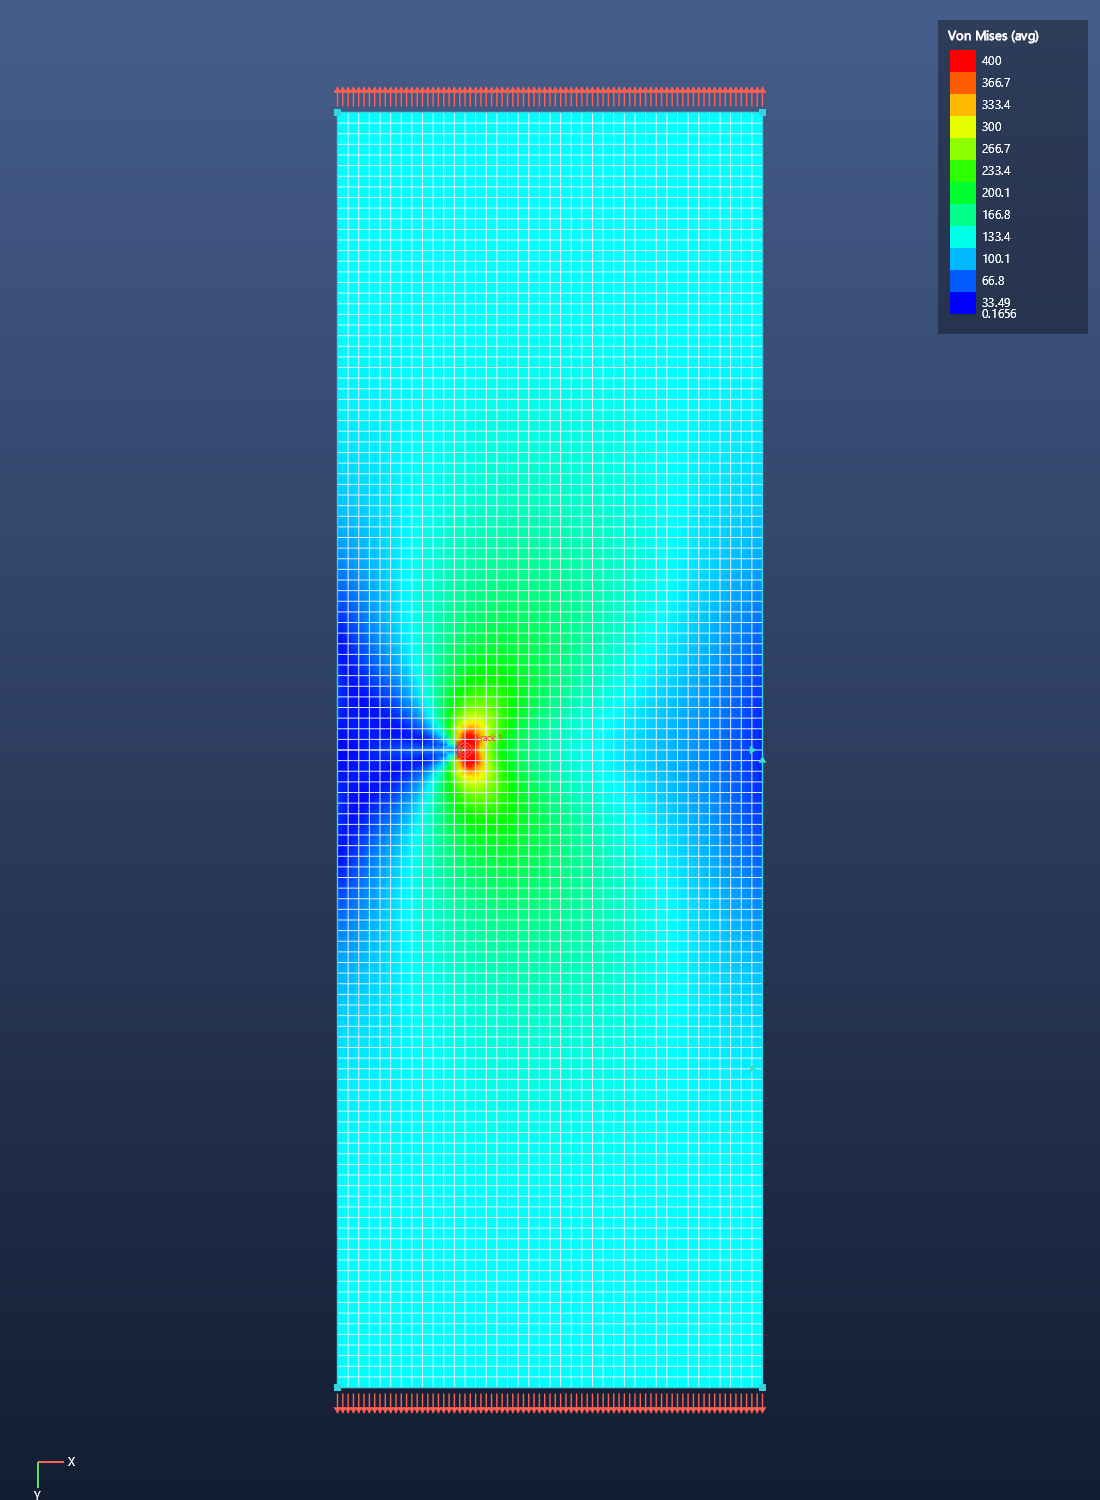
\includegraphics[height=9.2cm]{crack-sent-vm.png}\hspace{4mm}
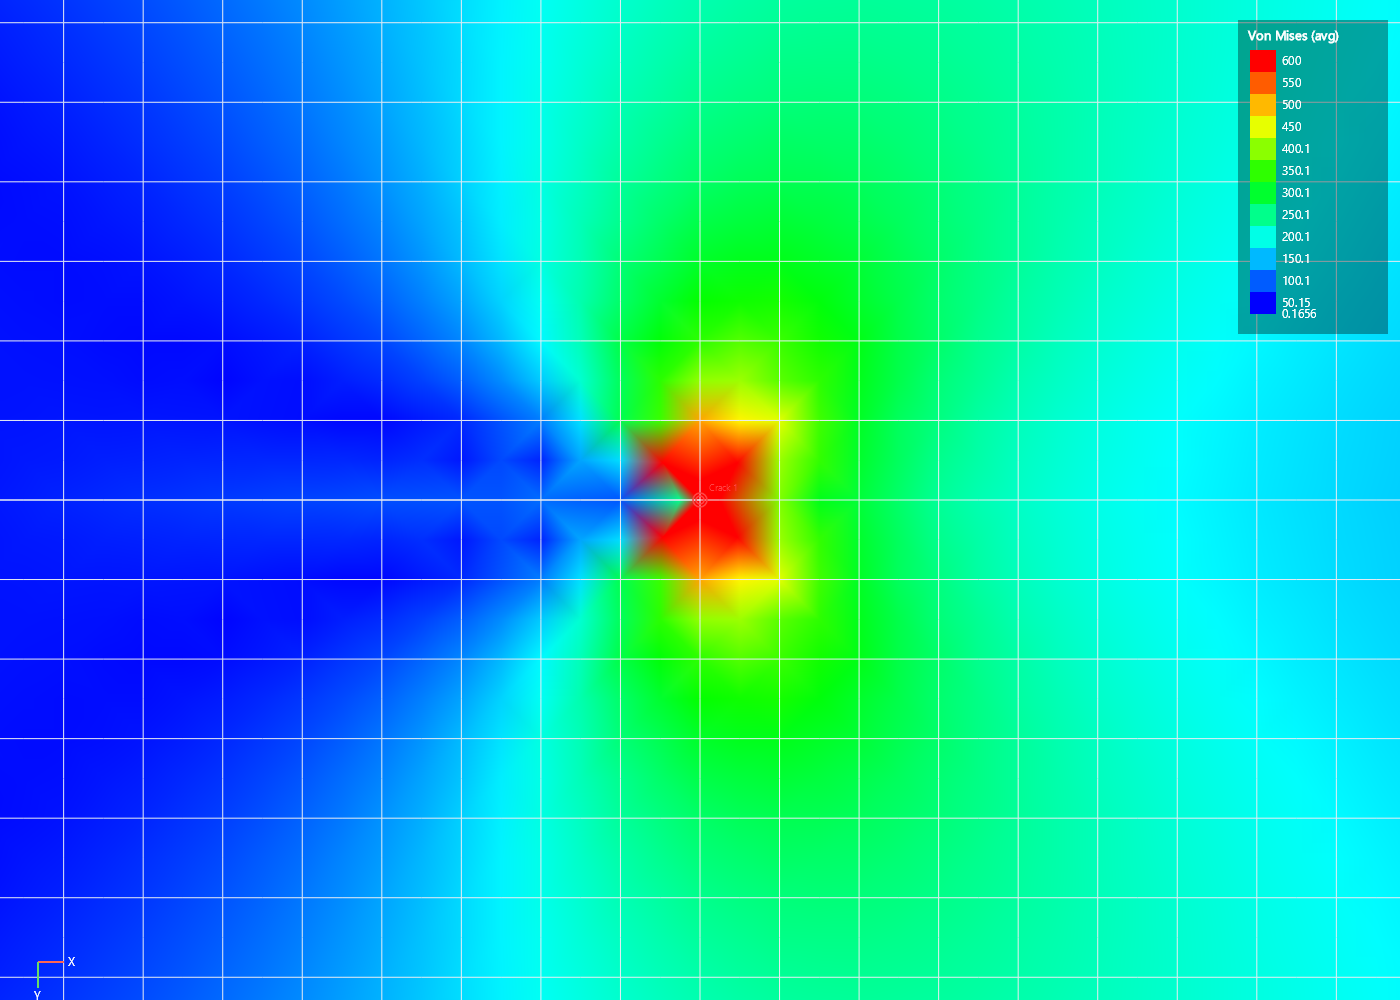
\includegraphics[height=9.2cm]{crack-sent-tip-zoom.png}
\caption{K1: SENT von Mises field (legend capped for display) and tip
close-up showing the characteristic lobed field and unloaded crack wake.}
\end{figure}

\begin{table}[H]\centering\small
\begin{tabular}{@{}lcccc@{}}
\toprule
Quantity & Handbook & FEA Membranes & Error & NASTRAN CQUAD8R \\
\midrule
$K_I$ (interaction integral) & 510.3 & 509.7 & $-0.1\,\%$ & \nast \\
$K_I$ (displacement correlation) & 510.3 & 534.6 & $+4.8\,\%$ & --- \\
$K_{II}$ & 0 & $\approx0$ & $<2\,\%$ of $K_I$ & \nast \\
\bottomrule
\end{tabular}
\caption{K1 results (test \texttt{Crack\_EdgeCrackedPlate\_MatchesHandbookK1}).}
\end{table}

\section{K2 --- Centre-cracked tension (CCT), both tips}
Plate $20\times40$, half-crack $a=4$ ($a/W=0.4$), both tips created in one
command. Handbook (Feddersen): $K_I = \sigma\sqrt{\pi a\,\sec(\pi a/2W)} = 394.1$.

\begin{figure}[H]\centering
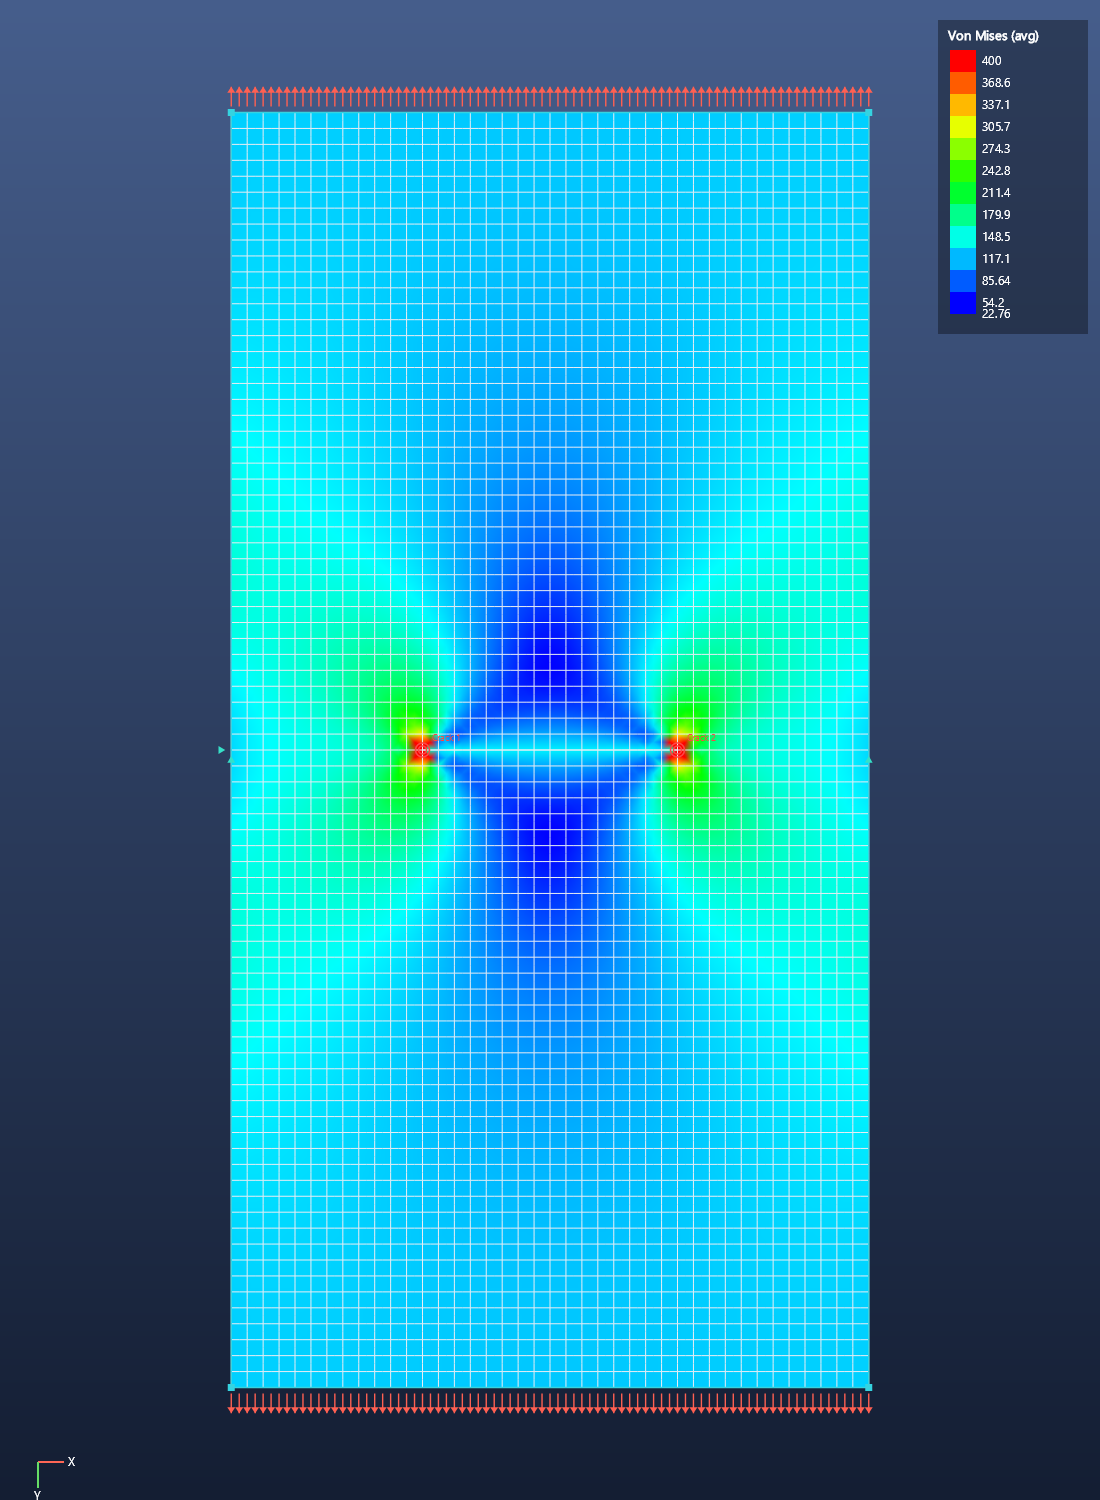
\includegraphics[height=9.2cm]{crack-cct-vm.png}\hspace{4mm}
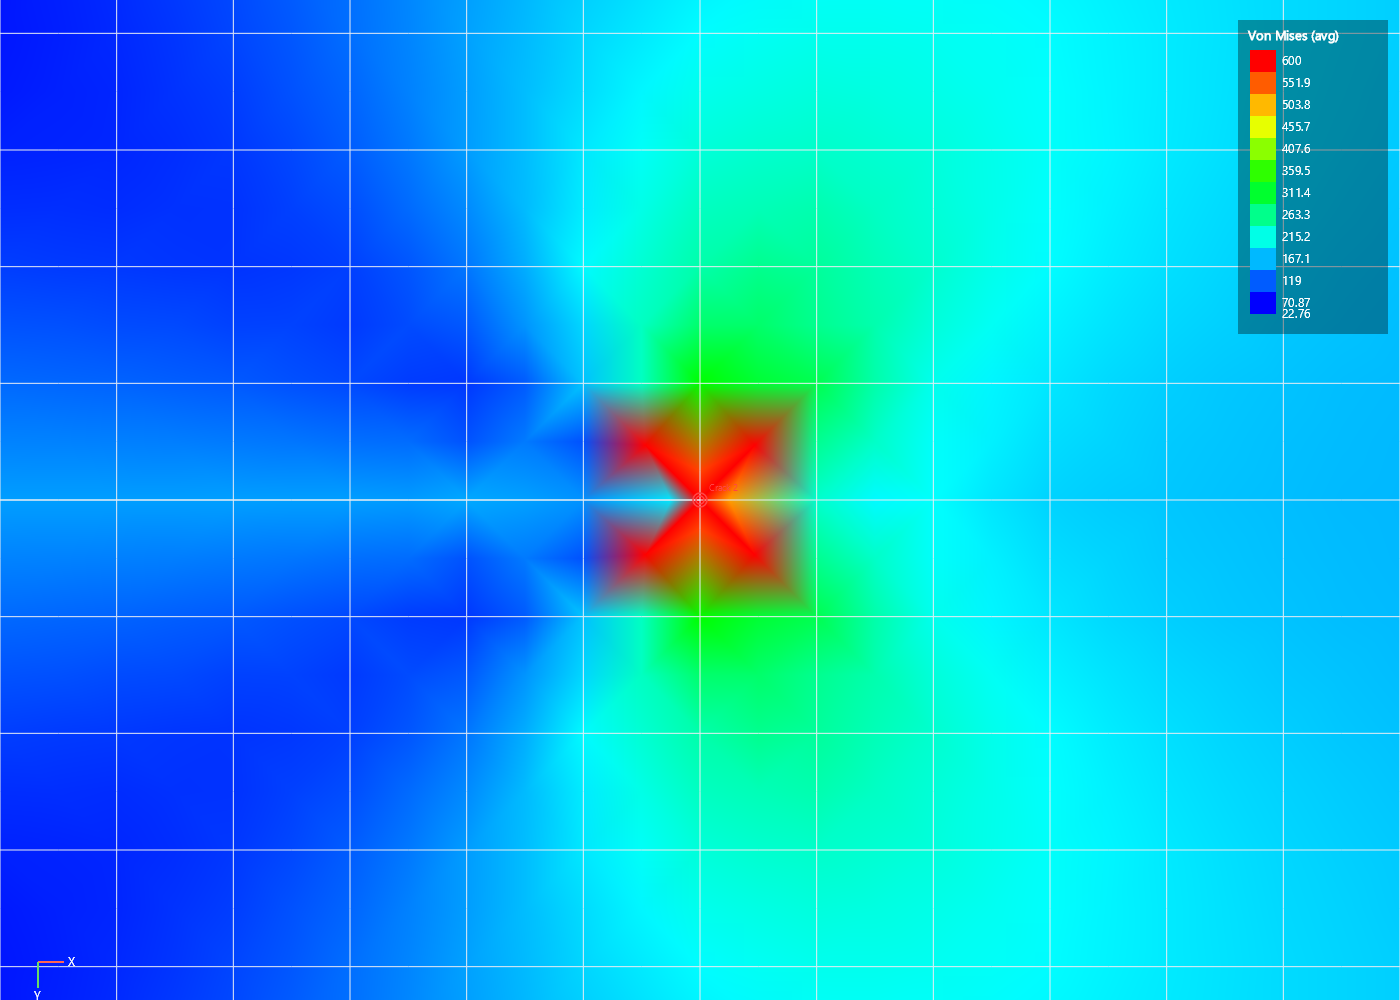
\includegraphics[height=9.2cm]{crack-cct-tip-zoom.png}
\caption{K2: CCT von Mises field and right-tip close-up.}
\end{figure}

\begin{table}[H]\centering\small
\begin{tabular}{@{}lcccc@{}}
\toprule
Quantity & Handbook & FEA Membranes & Error & NASTRAN CQUAD8R \\
\midrule
$K_I$ (interaction integral) & 394.1 & 393.7 & $-0.1\,\%$ & \nast \\
$K_I$ (displacement correlation) & 394.1 & 418.9 & $+6.3\,\%$ & --- \\
$K_{II}$ & 0 & $\approx0$ & $<2\,\%$ of $K_I$ & \nast \\
Tip symmetry & equal & equal & 1 decimal & \nast \\
\bottomrule
\end{tabular}
\caption{K2 results (test \texttt{Crack\_CentreCrackedPlate\_MatchesHandbookK1\_BothTips}).}
\end{table}

\section{K3 --- Domain independence}
The defining correctness property of a domain integral: the same SENT solution
evaluated over integration annuli of 2, 3, 4 and 6 tip-element lengths agrees
within \textbf{1\,\%} of the mean (test
\texttt{Crack\_InteractionIntegral\_DomainIndependence}).

\section{Method accuracy statement}
The interaction integral measures $-0.1\,\%$ on both handbook benchmarks and
is domain-independent to $<1\,\%$. The displacement-correlation cross-check
carries the known $\approx5\,\%$ bias of non-collapsed rectangular
quarter-point arrangements ($+5$ to $+6\,\%$ with the production
reduced-integration Q8). In application work, a large divergence between the
primary $K$ and the DCT value should prompt inspection of the tip mesh.

% =====================================================================
\chapter{Diagnostics and model-integrity verification}
\label{sec:diagnostics}
% =====================================================================

\begin{itemize}
  \item \textbf{Orphan nodes}: a pre-solve check names any node with no
        attached stiffness instead of failing opaquely.
  \item \textbf{Under-constrained models}: the sparse LU factorisation does
        not necessarily fail on a singular matrix; every solution is therefore
        verified against $\lVert Ku-f\rVert \le 10^{-6}\lVert f\rVert$ and
        rigid-body mechanisms are rejected with a clear message. (This guard
        exists because testing caught the factorisation returning silent
        zeros.)
  \item \textbf{Editing integrity} (16 automated cases): re-meshing fully
        replaces meshes; deletion of nodes/elements/surfaces cascades to
        everything referencing them; coincident-node merging never destroys
        spring-joined fastener pairs nor heals crack faces; RBE2 and crack
        records are remapped or pruned through all operations; the webtool
        JSON format round-trips.
\end{itemize}

% =====================================================================
\chapter{NASTRAN comparison programme}
% =====================================================================

The grey dashes throughout this manual are reserved for MSC~NASTRAN results
using CQUAD8(R) elements on identical meshes. Recommended procedure per case:

\begin{enumerate}
  \item Open the benchmark model (\texttt{validation/*.json}) in FEA Membranes
        and export the results CSV (\emph{File $\to$ Export Results as CSV});
        the NODES section gives the exact node coordinates for the NASTRAN
        deck, and the BC columns give the constraint/load sets.
  \item Reproduce mesh, constraints and consistent loads in NASTRAN
        (CQUAD8 + PSHELL membrane-only, or CQUAD8R where available); for the
        crack cases use the same quarter-point node positions (the CSV
        coordinates already include the quarter-point shifts).
  \item Record tip deflections / stresses / $K$ values in the comparison
        columns; note the NASTRAN version, element keyword and any parameter
        settings (e.g.\ K6ROT, SNORM defaults are irrelevant for membranes)
        beside each table.
\end{enumerate}

% =====================================================================
\appendix
\chapter{Reproduction}
% =====================================================================

\section*{A.1 Run the automated suite}
\begin{verbatim}
dotnet test tests/FeaCore.Tests/FeaCore.Tests.csproj
\end{verbatim}
46/46 cases pass at this revision. The suite also regenerates every benchmark
model into \texttt{validation/}.

\section*{A.2 Regenerate the figures}
\begin{verbatim}
FeaMembranes.exe --render <model.json> <out.png>
    [--contour vm|sx|sy|sxy|none] [--deformed] [--no-nodes]
    [--vectors springs|reactions|both] [--cmax <value>]
    [--zoom <cx> <cy> <halfwidth>] [--width N] [--height N]
\end{verbatim}
The exact commands used for the figures in this manual are recorded in
\texttt{validation/img/render-commands.ps1}.

\section*{A.3 Automated test inventory}
The complete case-by-case record, with per-test acceptance tolerances, is
maintained in \texttt{validation/VALIDATION.md} (kept current by construction:
a failing case fails the build).

\end{document}
